\documentclass{standalone}
\usepackage{tikz}
\begin{document}
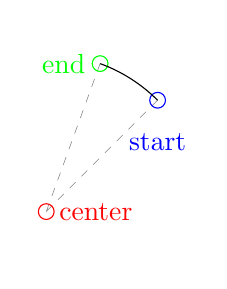
\begin{tikzpicture}
\def\x{3}
\def\y{1}
\def\start{45}
\def\stop{70}
\def\radius{2}
\coordinate (start) at (\x,\y);
\coordinate (center) at ({\x-\radius*cos(\start)},
                         {\y-\radius*sin(\start)});
\coordinate (end) at ({\x-\radius*cos(\start)
                         +\radius*cos(\stop)},
                      {\y-\radius*sin(\start)
                         +\radius*sin(\stop)});
\draw[help lines,dashed] (center) -- (start) (center) -- (end);
\draw[circle,blue] (start) circle (.1) node[below]{start};
\draw[circle,red] (center) circle (.1) node[right]{center};
\draw[circle,green] (end)  circle (.1) node[left]{end};

\draw (\x,\y) arc (\start:\stop:\radius);

\end{tikzpicture}
\end{document}
